% =============================================================================
% sem_revised_v1.tex — first revision draft
% Modeling Pragmatic Reasoning behind Social Meaning
% Target venue: Meaning: A Journal of Linguistics and Philosophy
% Plain article class — switch to journal template after acceptance.
% =============================================================================
\documentclass[12pt,a4paper]{article}

% --- Core packages -----------------------------------------------------------
\usepackage[T1]{fontenc}
\usepackage[utf8]{inputenc}
\usepackage[english]{babel}
\usepackage{amsmath}
\usepackage{amssymb}
\usepackage{graphicx}
% Notebook-generated figures live in ../figures/generated/ (produced by
% notebooks/sem_paper.ipynb). Re-running the notebook refreshes them automatically.
\graphicspath{{figures/}{../figures/generated/}}
\usepackage{booktabs}
\usepackage[margin=2.5cm]{geometry}
\usepackage{setspace}
\usepackage{caption}
\usepackage{float}
\doublespacing

% Float placement tuning (counters double-spacing crowding)
\renewcommand{\topfraction}{0.9}
\renewcommand{\textfraction}{0.1}
\renewcommand{\floatpagefraction}{0.8}
\setcounter{topnumber}{4}
\setcounter{totalnumber}{5}

% --- Bibliography (biblatex) -------------------------------------------------
\usepackage[backend=bibtex,
            style=authoryear,
            sortcites=true,
            sorting=nyt,
            dashed=false,
            natbib]{biblatex}
\addbibresource{mybib.bib}

% --- Hyperlinks --------------------------------------------------------------
\usepackage[hidelinks]{hyperref}

% --- Linguistic examples -----------------------------------------------------
\usepackage{linguex}
\renewcommand{\firstrefdash}{}

% --- Semantic brackets -------------------------------------------------------
\usepackage{stmaryrd}
\newcommand{\sem}[2][]{\ensuremath{\llbracket#2\rrbracket^{#1}}}
\newcommand{\type}[2]{\ensuremath{\langle #1,#2 \rangle}}

% --- Convenience macro for small caps attribute names ------------------------
\newcommand{\xvar}[1]{\textsc{#1}}

% =============================================================================
\title{Modeling Pragmatic Reasoning behind Social Meaning}
\author{[Anonymous for review]}
\date{}

% =============================================================================
\begin{document}
\maketitle

\begin{abstract}
Researchers are increasingly interested in how pragmatic reasoning influences
the social impressions we form of a speaker. This study examines the complex
interplay between language use, situational context, pragmatic inference, and
social meaning. The Social Evaluation Model (SEM) is presented, a probabilistic
framework that models how listeners form social judgments about speakers based
on their linguistic choices and the situational context, by reasoning about the
speaker's knowledge states and communicative motivations. We situate SEM within
the broader tradition of probabilistic pragmatics, showing how it extends the
inferential chain of the Rational Speech Act framework to social evaluation as
an explicit target of inference. We test the model's predictions against data
from a matched-guise experiment on numerical (im)precision, evaluating both its
qualitative and quantitative fit to human social judgments. Our findings
contribute to existing research in
sociolinguistics and formal pragmatics, providing a principled probabilistic
framework for understanding how linguistic choices convey social meaning through
pragmatic inference.
\end{abstract}

\noindent\textbf{Keywords:} social meaning, pragmatic inference, social
evaluation, probabilistic pragmatics, Rational Speech Act, numerical precision

% -----------------------------------------------------------------------------
\section{Introduction}
% -----------------------------------------------------------------------------

\subsection{From Gricean Maxims to Probabilistic Pragmatics}

The study of pragmatic inference, how listeners derive meaning beyond the
literal words, began with H.~P.~Grice's influential work on implicature
\citep{grice}. Grice proposed that conversation follows a \emph{Cooperative
Principle} along with maxims that speakers typically adhere to for effective
communication. When a speaker seemingly violates a maxim, the listener assumes
cooperation and infers an additional layer of meaning, known as
\emph{implicature}. This framework established that meaning relies on
\emph{rational inference} regarding the speaker's intent. Building on Grice's
foundation, \citet{horn1989} and \citet{levinson2000} introduced
\emph{neo-Gricean} models, refining the types of implicature and incorporating
scalar reasoning (e.g., ``some'' suggesting ``not all''). These early theories
demonstrated that pragmatic inference involves not just language but also social
reasoning, shaped by expectations of cooperation and relevance.

Gricean pragmatics initially focused on cooperative reasoning, but later
developments began to view implicature as indicative of the speaker's epistemic
state: what the speaker knows, believes, or is committed to. A central insight of
this tradition is that deriving a strong (``not all'') inference from a weaker
form requires more than the assumption of cooperativity; it requires an
additional \emph{competence assumption}, namely that the speaker is informed
about whether the stronger alternative holds \citep{sauerland2004,schulzvanrooij2006,geurts2010}.
Without this assumption, an underinformative utterance licenses only a weak
\emph{ignorance} inference (the speaker does not know that the stronger
alternative holds); with it, the listener can strengthen this to the conclusion
that the speaker knows it to be false. This move from primary to secondary
implicature, the \emph{epistemic step} \citep{sauerland2004,BrehenyKatsosWilliams2006},
makes explicit that pragmatic enrichment is driven by the listener's model of the
speaker's knowledge, not by the utterance alone. The scalar case is the classic
illustration \citep{Spector2007,ChemlaSingh2014a}: whether ``some'' implies ``not
all'' depends on whether the speaker is taken to know the stronger alternative to
be false or merely fails to affirm it. More broadly, this represented a shift from
truth-conditional to epistemic interpretations of pragmatic reasoning, in which
the listener's inference is fundamentally an inference about the speaker's mind.

Probabilistic and Bayesian
models, including the Rational Speech Act (RSA) framework
\citep{frank2012,GoodmanStuhlmuller2013,PottsLassiterLevyFrank2016}, advanced
this perspective by conceptualizing pragmatic inference as Bayesian reasoning
over the speaker's epistemic beliefs and communicative goals. From this
viewpoint, pragmatic inference is nuanced and probabilistic, reflecting
uncertainty about the speaker's knowledge and intentions.

\subsection{Intentions, Motives, and Communicative Goals}

Beyond epistemic reasoning, a substantial body of work locates pragmatic
inference in the recovery of speaker intentions and motives: the \emph{why}
behind an utterance. The foundations are philosophical. \citet{Grice1957} defined
speaker meaning itself in terms of intention recognition: a speaker means
something by an utterance in virtue of intending the hearer to recognize that
very intention, so that understanding an utterance is, at bottom, an inference
about the speaker's communicative intentions. \citeauthor{SperberWilson1995}'s
(\citeyear{SperberWilson1995}) Relevance Theory develops this into a cognitive
account on which comprehension is the search for an interpretation that the
speaker could rationally have intended to be optimally relevant, recovering both
the speaker's informative intention (what they aim to convey) and their
communicative intention (that they aim to convey it). On these views, inference
about meaning is inseparable from inference about why the speaker spoke as they
did.

Crucially, the relevant motives are often \emph{social} rather than purely
informational. \citeauthor{brownlevinson1987}'s (\citeyear{brownlevinson1987})
politeness theory casts utterance choice as the management of face, and work in
developmental and cognitive pragmatics treats communication as fundamentally
cooperative social action \citep{Tomasello2003,Clark1996}. The clearest
illustration that speakers choose forms strategically comes from research on
indirect speech: \citet{LeePinker2010} explain off-record indirectness through a
``strategic speaker'' who trades efficiency for plausible deniability when
unsure whether the hearer is cooperative or antagonistic, on the premise that
communication mixes cooperation with conflict and that language serves both to
convey information and to negotiate the speaker--hearer relationship. What such
work establishes, and what matters for the model developed below, is that the
choice of one form over an available alternative is itself an object of
inference: listeners routinely ask not only what a speaker meant but why they
chose to mean it \emph{that way}, and they draw conclusions about the speaker
accordingly.

Recent computational and cognitive models bring the epistemic and intentional
strands together, treating pragmatic interpretation as joint Bayesian reasoning
about what the speaker knows and what they are trying to do. 
RSA models the listener as inverting a model of a
goal-directed speaker \citep{frank2012,goodman2016},
and \citet{bergen2016} show how reasoning over
semantic alternatives and speaker goals can be combined within a single
probabilistic system. Extensions to explicitly social goals, such as
\citeauthor{yoontessleretal2020}'s (\citeyear{yoontessleretal2020}) model of
polite speech, demonstrate that listeners jointly infer informational and social
intentions from a single utterance. This convergence reflects a broader trend in
contemporary pragmatics toward integrating informational (epistemic) and
intentional (motivational) reasoning within one social-cognitive process,
precisely the integration the present model builds on.


\subsection{The Role of Context}

Both strands of pragmatic reasoning surveyed so far, the epistemic and the
motivational, operate under the control of context. A large experimental
literature shows that even the most-studied inferences are not computed
automatically but depend on the situation: scalar implicatures arise more
readily when the context makes the stronger alternative relevant, and recede
when it does not \citep{BrehenyKatsosWilliams2006,DegenTanenhaus2015}. A
recurring way of articulating this dependence is through the \emph{Question Under
Discussion}: context fixes which alternatives are live, and hence which
inferences a listener is licensed to draw \citep{roberts2012}. More generally,
\citet{vanRooij2003} and \citet{Clark1996} stress that pragmatic reasoning
unfolds within common ground and joint activity, so that the same utterance can
support different inferences depending on the conversational situation. Context,
on this view, is not a backdrop but a determinant of pragmatic meaning: it sets
the alternatives, the relevant question, and the assumptions against which an
utterance is interpreted.

This context-sensitivity is not peculiar to epistemic inference. As the next
subsection develops, the \emph{social} meaning a listener reads off a speaker's
choice is equally situation-dependent: the same linguistic form can support
different social interpretations in different contexts, rather than carrying a
fixed social value \citep{campbellkibler2007}. It is this shared property, that both what a speaker is taken
to know and how they are socially evaluated depend on the context of utterance,
that the model developed in this paper builds on, treating social evaluation as a
context-sensitive inference of the same general kind that governs epistemic
interpretation.

\subsection{Social Meaning and Pragmatic Reasoning}

Research in sociopragmatics explores how pragmatic reasoning interacts with
\emph{social meaning}: the constellation of qualities and properties that
linguistic forms convey about the social identity of their users, including
demographic traits, personality characteristics, and ideological orientations
\citep{beltrama2020,Eckert2008,Podesva2011,Silverstein2003}. The study of
social meaning has its roots in variationist sociolinguistics.
\citeauthor{Labov1972}'s (\citeyear{Labov1972}) foundational work demonstrated
that linguistic variation is systematic and socially stratified, linking language
use to social structure and change. Subsequent research moved beyond correlating
variants with fixed demographic categories toward understanding how speakers
actively deploy variation to construct stances, styles, and personas;
\citeauthor{Eckert2012}'s (\citeyear{Eckert2012}) ``three waves'' synthesis
characterizes this trajectory, culminating in a view on which social meaning is
not a static property of a form but is produced in interaction.

A central concept in this tradition is the \emph{indexical field}
\citep{Eckert2008,Silverstein2003}: a constellation of ideologically related
potential meanings associated with a linguistic form, only some of which are
activated on any given occasion depending on the speaker, the listener, and the
situation. \citet{campbellkibler2007} demonstrates this empirically: the English
variable (ING) shifts listeners' perceptions along dimensions such as education,
articulateness, and formality, but its effect is not constant. The same variant
can be heard as compassionate or condescending depending on the listener's prior
orientation to the speaker; even a personality trait as seemingly stable as
\emph{educated} is perceived differently across contexts and listeners.
What is indexed is thus not a fixed social value but a field of potential
meanings, and what counts is the perception, not the attribute itself. This
is the context-sensitivity anticipated at the end of the previous subsection:
social meaning, like epistemic meaning, is the product of situated interpretation
rather than a fixed mapping from form to value.

Two routes by which social meaning arises can be distinguished. In the first,
social meaning is tied directly to the \emph{form}: a variant acquires indexical
associations through repeated co-occurrence with speakers who embody certain
social characteristics, a process known as enregisterment
\citep{agha2003,campbellkibler2007}. The classic cases are sociophonetic
variables whose alternants do not differ in truth-conditional content ---
for Labov, it is precisely truth-conditional \emph{equivalence} that creates
the space for social meaning to arise, since variant choice has no consequences
for what is said \citep{terkourafi2026}. In the second route, social meaning
arises from the \emph{reasoning process}: a listener infers attributes about a
speaker by reasoning about why they chose one form over its alternatives, in
much the same way that pragmatic implicatures arise from reasoning about
cooperative communication \citep{Acton2019,beltramapapafragou2023,soltEtAl2025}.
On this account, it is precisely the \emph{difference} in content between
alternatives that triggers the inference: because the alternatives convey
different information, the speaker's choice among them constitutes evidence about
their epistemic state and communicative motivation \citep{terkourafi2026}.

The two routes produce social meanings with distinct properties
\citep{terkourafi2026,burnett2026}. Form-based social meanings are typically
non-cancellable (the Vineyarder accent means ``Vineyarder'' even if the speaker
disavows it), often ineffable, and subject to drift as indexical associations
shift over time and place. 
Reasoning-based social meanings, by contrast, are propositional (the inference
can be stated) and cancellable (a speaker can explicitly rule out a motivation),
since they are derived from general principles of rational communication rather
than from community-specific enregistered links between form and identity.
These are not two disjoint categories but poles of a continuum \citep{Eckert2019}.

Several strands of work develop the idea that social attributes are derived
inferentially from a speaker's pragmatic choices, rather than read off the form
directly. \citet{Acton2019} shows that even a function word like the definite
article carries social meaning through the stance it signals toward a referent,
and \citet{actonhunt2025} demonstrate that the choice between a singular
definite (\emph{the family}) and a possessive (\emph{your family}) conveys a
distinctive social stance through competition with alternatives. Closest to the
present study, \citet{beltramaetal2022} find that the choice between precise
and approximate numerical expressions leads listeners to distinct social
evaluations modulated by context, and \citet{beltramapapafragou2023} show that a
speaker's adherence to or violation of the Gricean maxims of Relevance and
Informativeness shifts perceptions of their warmth and competence. Critically,
the latter find that the social effect depends on the inferred \emph{reason}
for the speaker's behavior: an uninformative answer attributed to inability is
evaluated differently than one attributed to unwillingness. This is precisely
the inferential route from pragmatic choice to social evaluation that the
present work sets out to formalize.




%COMMENTS:
%MORE EXAMPLES ON SOCIAL MEANING
%NDEXICAL: CLUSTER OF RELATED MEANINGS RELATED TO THE FORM
%LOOK AT HEATHERS SUMMARY - BELTRAMAS OVERVIEW PAPER DEFINITION
%BE CLEARER ON SOCIOLINGUISTIC TERMONOLOGY
%IS STATIC OR DYNAMIC THE CORRECT TERM HERE?
%BE CLEARER ON THE DIFFERENCE BETWEEN INDEXICAL AND ATTRIBUTE-BASED SOCIAL MEANING
%WHAT IS SPECIAL ABOUT THE ATTRIBUTES WE CARE ABOUT?
%ON SOCIONLINGUISTIC LITERATURE TEHRE IS PLENTY OF DYNAMIC ATTRIBUTES (E.G. passionate, ...)
%EVEN IF THE ATTRIBUTE IS NOT DYNAMIC - THE PERCEPTION CAN BE
%WHAT COUNTS IS THE PERCEPTION, NOT THE ATTRIBUTE ITSELF  
%WHAT COUNTS: SOCIAL MEANING TIGHT TO THE FORM VS SOCIAL MEANING RISES ABOUT THE REASONING PROCESS (SHOULD BE HERE!!!)
%SOCIAL MEANING COMES FROM REASOING ABOUT FORMS
%FORMS THAT ARE NOT  
%HEATHER SHOWS MANY EXAMPLES WHERE ALTERNATIVES DO NOT DIFFER IN THEIR CORE-SEMANTIC MEANING!!!
%ALTERNATIVES THAT ARE NOT CORE_MEANING EQUIVALENT
%CHECK FOR THE TERM ATTRIBUTE_BASED AND ATTRIBUTE_LEVEL (SINCE THIS IS NOT SPCIAL TO THE PHENOMENON)
%DISCUSSION: EQUIVALENT ALTERNATIVES...
%HEATERS MODEL ATTACHES SOCIAL MEANING TO THE FORM, BUT NOT THE REASONING PROCESS



\subsection{The Present Work}

Taken together, these developments reveal that pragmatic understanding is a form
of social cognition: to interpret an utterance, a listener reasons jointly about
what the speaker knows, why they chose to speak as they did, and what this
implies about them as a social agent, all under the control of context. What has
so far been established largely through separate experimental and theoretical
strands, however, has not been brought together in a single explicit model of how
these inferences combine to yield a social evaluation.

Building on these insights, we introduce the Social Evaluation Model (SEM), a
probabilistic framework that formalizes how linguistic choices, situational
context, and pragmatic reasoning work together to shape listeners' social
judgments. SEM shows how listeners infer a speaker's knowledge state and
communicative motivation from their language use, and how these inferences give
rise to evaluations of social attributes such as competence, helpfulness, and
likability. The framework expands the inferential chain of probabilistic
pragmatics to include evaluative meaning, where small differences in language
use can lead to subtle, context-dependent changes in social interpretation
\citep[e.g.,][]{beltramapapafragou2023}.

The paper is organized as follows. Section~\ref{sec:sem} provides a formal
definition of the SEM, situating it within the probabilistic pragmatics
tradition and comparing it to the RSA framework. A case study on numerical
(im)precision is used to develop and qualitatively evaluate the model in
Section~\ref{sec:imprecision}. Section~\ref{sec:evaluation} presents a
quantitative evaluation of the model's predictions, including a comparison of
the full model against nested ablations. Section~\ref{sec:conclusion} discusses
the model's contributions and directions for future work.


% -----------------------------------------------------------------------------
\section{The Social Evaluation Model}
\label{sec:sem}
% -----------------------------------------------------------------------------

%COMMENTS
%EMPASIS ON COMPARISONS TO RSA
%AT THE BEGINNING GOOD
%LATER IT REAPPEARS
%REDUNDENCIES WTH COMAPRING TO RSA
%REMOVE RSA COMPARISON AT THE POIT AFTER THE MODEL


\subsection{From Meaning Recovery to Social Evaluation}

The Social Evaluation Model (SEM) is a probabilistic framework for predicting
how listeners form social judgments about speakers based on their linguistic
choices. It builds on the core architecture of probabilistic pragmatics, in
particular the Rational Speech Act framework \citep{frank2012,goodman2016} and
the broader tradition of Bayesian pragmatic modeling surveyed by
\citet{franke2016}, while extending that architecture toward a target of
inference that has not previously been formalized within it: the social
evaluation of the speaker as a communicative agent.

Like RSA and related models, SEM treats pragmatic interpretation as Bayesian
inference. A listener who hears utterance $u$ in context $c$ does not simply
decode its semantic content; they reason probabilistically about what mental
states could have produced that utterance. Central to this reasoning is a set of
utterance alternatives $U$, the other things the speaker could have said, and
a commitment to the truthfulness constraint, which limits the knowledge states a
speaker could plausibly be in given what they actually said. These features are
not incidental borrowings from RSA; they are load-bearing components of SEM, and
the model's predictions depend on them in the same structural way RSA predictions
do (Figure~\ref{fig:sem_rsa}, left).

\begin{figure}[t!]
  \centering
  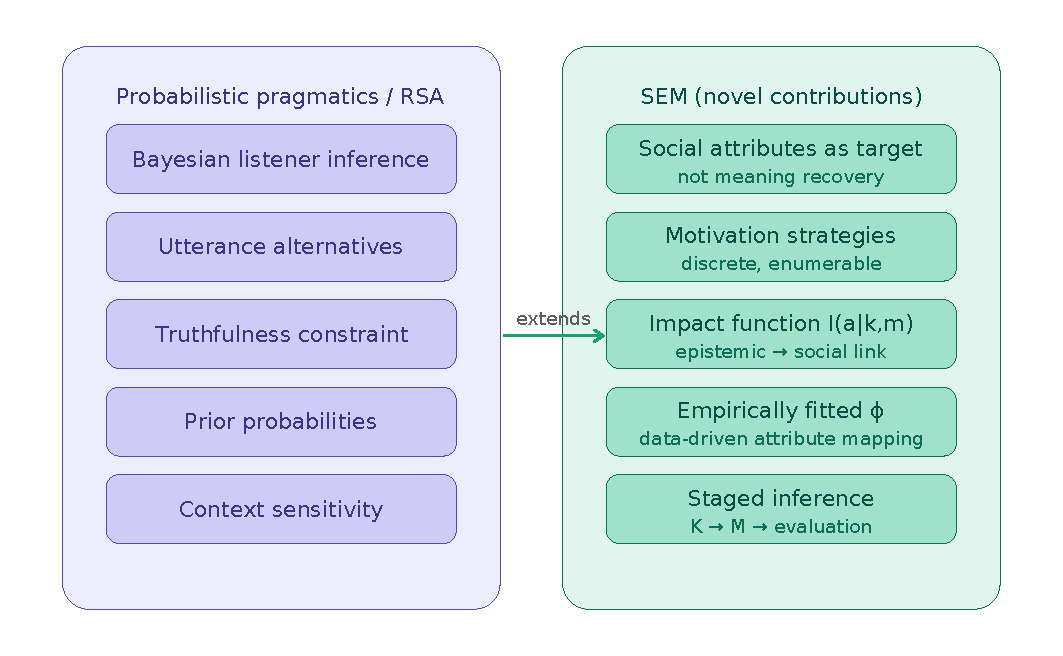
\includegraphics[scale=0.8]{figures/semRSArelationship.pdf}
  \caption{The relationship between Probabilistic Pragmatics / RSA and the
           Social Evaluation Model (SEM). SEM extends the core components of
           RSA (Bayesian listener inference, utterance alternatives,
           truthfulness constraint, prior probabilities, and context
           sensitivity), with novel components: social attributes as the
           target of inference, discrete motivation strategies, an impact
           function~$I(a \mid k, m;\omega)$ linking epistemic to social
           dimensions, empirically fitted trivalent functions~$\phi$, and
           staged inference ($u,c \to K \to M \to a$).}
  \label{fig:sem_rsa}
\end{figure}

Where SEM departs from existing probabilistic pragmatic models is in what the
listener is ultimately trying to infer. In RSA, inference terminates at meaning:
the listener recovers the speaker's intended message. In SEM, meaning recovery is
not the endpoint but an intermediate step. The listener uses their inferences
about the speaker's epistemic state, what the speaker knew and what they could
therefore truthfully have said, to make a further inference about the speaker's
communicative motivation: why did they choose this utterance over its
alternatives? And from that motivational inference, together with the inferred epistemic
state itself, the listener arrives at a social evaluation: what does this choice
reveal about the speaker's competence, helpfulness, or friendliness?

This reasoning, inferring the knowledge state from the utterance, then the
motivation from the knowledge state and context, is what SEM formalizes; the
social attribute is then evaluated from both the inferred knowledge state and the
inferred motivation jointly. The
key novel components, relative to RSA, are: (i)~social attributes as an explicit
target of inference; (ii)~discrete motivation-based strategies, each of which determines, 
for a given context and knowledge state, which out of a set of possible utterances
 a speaker will use; (iii)~an impact
function $I(a|k,m;\omega)$ that links epistemic and motivational inferences to
graded social evaluations; and (iv)~empirically fitted trivalent functions that
specify the direction of each inference-to-evaluation link. 
%There is no
%counterpart to this function in standard RSA, because RSA does not model social
%evaluation as an output. 
Figure~\ref{fig:sem_rsa} provides an overview of the
shared and novel components, and Figure~\ref{fig:sem_net} shows the full model
as a Bayesian network.



\begin{figure}[t!]
  \centering
  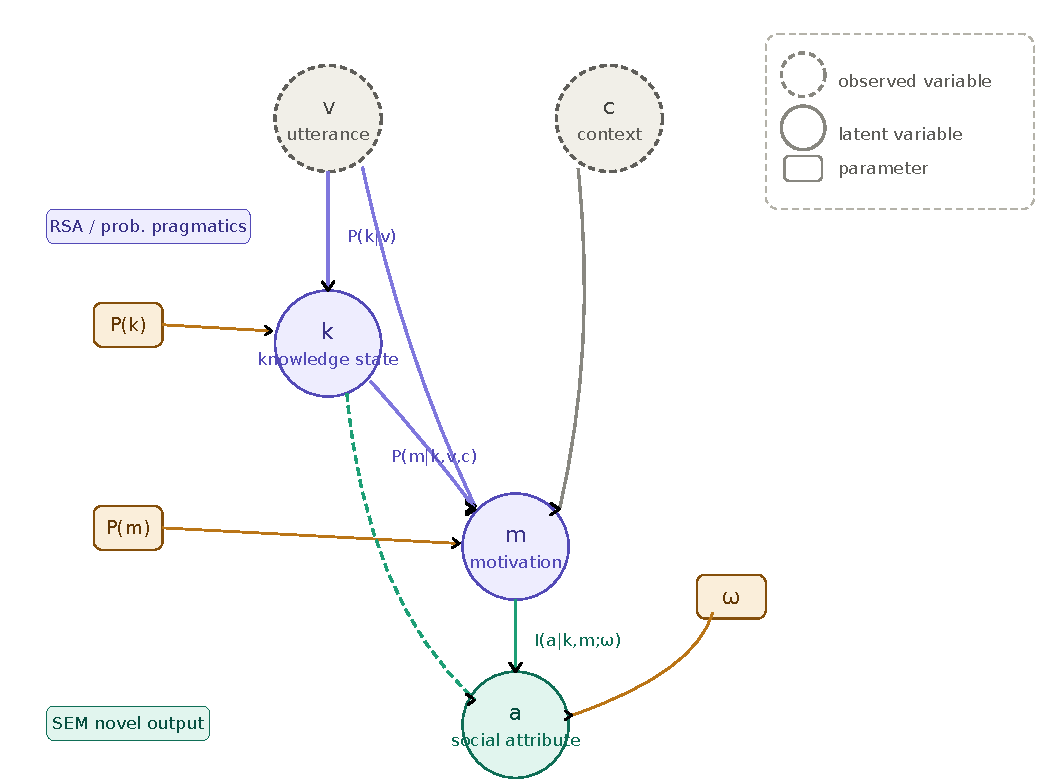
\includegraphics[scale=0.9]{figures/semNet.pdf}
  \caption{Bayesian network representation of the Social Evaluation Model.
           Dashed circles denote observed variables (utterance $u$, context $c$)
           available to the listener. Solid circles denote latent variables
           inferred by the listener: knowledge state $k$, motivation-based
           strategy $m$, and evaluation of the social attribute $a$. Rectangles denote
           free parameters: prior probabilities $P(k)$ and $P(m)$, and the
           weight parameter $\omega$. Inference proceeds in three stages:
           $u$ and $P(k)$ jointly determine the posterior over knowledge states
           $P(k|u)$; $k$, $u$, $c$, and $P(m)$ determine the posterior over
           strategies $P(m|k,u,c)$; and $k$ and $m$ feed into the impact
           function, weighted by $\omega$, to yield the social evaluation of attribute $a$.}
  \label{fig:sem_net}
\end{figure}


%\subsection{The Model Architecture}


%%The social evaluation model\footnote{A Python implementation of SEM, including a 
%reviewer-facing Jupyter
%notebook that reproduces the computations and figures in this paper, is available
%at \url{[ANONYMIZED GITHUB REPO LINK]}.}
%(SEM) predicts the listener's social assessment of the speaker based on using
%utterance $u$ from a set of alternatives $U$, given a situational context
%$c \in C$. Formally, the listener's evaluation function
%$E_L(a|u,c)$,\footnote{The function is defined as $E_L: A \times U \times C
%\rightarrow \mathbb{R}$; it returns a numerical score representing the
%listener's evaluation of the speaker on attribute $a$.} which specifies how
%the listener evaluates a speaker concerning social attribute $a$, is defined as:


\subsection{The Model Architecture}

The core theoretical claim developed in the preceding section is that a
listener's social evaluation of a speaker follows from a staged inferential
process: hearing an utterance in context, the listener first asks \emph{what
could the speaker have known?}, and \emph{why did they choose this utterance
over its alternatives?}, and finally \emph{what does that combination of
knowledge and motivation reveal about them as a communicator?} SEM formalizes
each stage as a probabilistic inference, and the three components of the model
correspond directly to these three questions: the knowledge-state inference
$P(k|u)$, the motivation inference $P(m|k,u,c)$, and the impact function
$I(a|k,m;\omega)$ that translates the inferred epistemic and motivational states
into a graded social evaluation.

Concretely, the listener's evaluation function
$E_L(a|u,c)$,\footnote{The function is defined as $E_L: A \times U \times C
\rightarrow \mathbb{R}$; it returns a numerical score representing the
listener's evaluation of the speaker on attribute $a$. A Python implementation
of SEM, including a Jupyter notebook that reproduces the computations and
figures in this paper, is available at \url{[ANONYMIZED GITHUB REPO LINK]}.}
which specifies how the listener evaluates a speaker on social attribute $a$
given utterance $u$ and context $c$, is defined as:

\begin{equation}
E_{L}(a|u,c) = \sum_{k \in K} \sum_{m \in M}
  P(k|u) \cdot P(m|k,u,c) \cdot I(a|k,m;\omega)
\label{eq1}
\end{equation}

\noindent where $K$ is a set of speaker knowledge states, and $M$ is a set of
motivation-based strategies, which are functions
that specify what utterance a speaker would produce across different contexts
and knowledge states when driven by a particular motivation.\footnote{Note: The same behavioral
strategy can in principle arise from different underlying motivations; the case
study in Section~\ref{sec:imprecision} provides detailed examples.} $P(k|u)$
and $P(m|k,u,c)$ are conditional probabilities, and $I(a|k,m;\omega)$ is an
impact function that determines how inferences about knowledge state and
motivation jointly affect the listener's evaluation of social attribute $a$.
The weight factor $\omega$ adjusts the relative contribution of epistemic versus
motivational inference to the evaluation. The evaluation function $E_L$ returns
a real number $x \in [-1, 1]$, where $x = -1$ indicates the lowest evaluation
and $x = 1$ the highest.\footnote{When a categorical judgment is required
(e.g., does the speaker possess attribute $a$ or not), one applies the sign
function: $x_{cat} = \mathrm{sgn}(x)$. For a probabilistic output, one applies
the sigmoid: $x_{prob} = (1 + e^{-\kappa x})^{-1}$, where $\kappa > 0$ controls
the steepness.}

\paragraph{Knowledge states and the truthfulness constraint.}
SEM considers situations in which a speaker chooses among \emph{non-equivalent}
alternatives: utterances that differ in their core-semantic meaning. The set $U$
represents exactly this --- the non-equivalent alternatives relevant in a given
situation. This is the first key assumption: because the alternatives in $U$
differ in what they assert, they differ in what knowledge states they are
compatible with.

The second key assumption is truthfulness: speakers only assert what they believe
to be true. Together, these two assumptions constrain what the listener can infer
about the speaker's epistemic state. When a speaker selects one alternative over
another, the listener can reason backwards: which knowledge states would have
permitted that utterance, and which would not? A speaker who uses a semantically
weaker form (e.g., ``some students passed'') may or may not know the stronger
fact; a speaker who uses a semantically stronger form (e.g., ``some but not all
students passed'') is committed to knowing it. The choice of utterance is
therefore direct evidence about what the speaker knew.

These different epistemic possibilities are represented by the set of knowledge
states $K$. The truthfulness constraint is implemented via a truthfulness
function $t: K \rightarrow \mathcal{P}(U)$, which maps each knowledge state $k$
to the set of utterances the speaker could truthfully produce in that state.
The posterior probability of knowledge state $k$ given utterance $u$ is then:

\begin{equation}
P(k|u) = \frac{P(k) \cdot \chi_t(k,u)}
               {\sum_{k' \in K} P(k') \cdot \chi_t(k',u)}
\label{eq2}
\end{equation}

\noindent where $P(k)$ is the prior probability of knowledge state $k$, and
$\chi_t(k,u) = 1$ if $u \in t(k)$ and $0$ otherwise.

\paragraph{Motivation-based strategies.}
Knowing what the speaker could have said is not yet sufficient to evaluate them
socially: two speakers in identical epistemic states may choose differently
depending on their communicative goals. The listener's second inferential task
is therefore to ask why the speaker chose this utterance over the alternatives
their knowledge permitted. SEM represents the space of possible answers as a
set $M$ of motivation-based strategies. Each strategy $m \in M$ is a function
$m: C \times K \rightarrow U$ that specifies the utterance a speaker would
choose in context $c$ with knowledge state $k$ when driven by a particular
motivation. For example, a maximally informative strategy always selects the
most informative available utterance given the current knowledge state, while a
speaker-convenience strategy always selects the least effortful form regardless
of context.

Given a set of strategies, the listener calculates $P(m|k,c,u)$, the
conditional probability that the speaker follows strategy $m$ given knowledge
state $k$, context $c$, and observed utterance $u$:

\begin{equation}
P(m|k,c,u) = \frac{P(m) \cdot \chi_m(c,k,u)}
                  {\sum_{m' \in M} P(m') \cdot \chi_m(c,k,u)}
\label{eq3}
\end{equation}

\noindent where $P(m)$ is the prior probability of strategy $m$, and
$\chi_m(c,k,u) = 1$ if $m(c,k) = u$ and $0$ otherwise.

\paragraph{The impact function.}
The impact function $I(a|k,m;\omega)$ defines how inferences about knowledge
state $k$ and motivation strategy $m$ affect the social evaluation on attribute
$a$. It captures the intuition that listeners' assumptions about what a speaker
knew and why they spoke as they did are systematically linked to evaluations of
social attributes. For example, inferring that a speaker 
was knowledgeable about the matter at hand 
may positively affect perceptions of competence, while inferring that a speaker
chose to omit relevant information may negatively affect perceptions of helpfulness.
Formally:

\begin{equation}
I(a|k,m;\omega) = \omega \cdot \phi_K(k,a) + (1-\omega) \cdot \phi_M(m,a)
\label{eq4}
\end{equation}

\noindent where $\phi_K: K \times A \rightarrow \mathbb{T}_3$ and
$\phi_M: M \times A \rightarrow \mathbb{T}_3$ are \emph{trivalent functions}
that indicate whether and how a knowledge state or motivation-based strategy
influences a social attribute.\footnote{A trivalent function maps inputs to one
of three values in $\mathbb{T}_3 = \{-1, 0, 1\}$, representing a significant
negative effect, no significant effect, or a significant positive effect
respectively. These values are fitted empirically from participant data, as
detailedin Section~\ref{sec:imprecision}.} The weight parameter $\omega \in
(0,1)$ controls the relative contribution of epistemic versus motivational
inference: high $\omega$ places more weight on what the speaker knew; low
$\omega$ places more weight on their inferred motivation.

A note on whose reasoning the model's free parameters encode. SEM has three
free parameters --- the prior probabilities $P(k)$ and $P(m)$ and the weight
$\omega$, shown as rectangles in the Bayesian network of
Figure~\ref{fig:sem_net} --- which are not determined by the model architecture
but must be set prior to inference.  Crucially, these parameters are properties of the \emph{listener}, not
the speaker: they specify how a particular listener distributes prior expectation
over knowledge states and motivations, and how heavily they weigh epistemic
against motivational inference in arriving at a social judgment. Different
listeners may bring different priors and weightings to the same utterance, and
SEM represents this variation directly through these parameters. The model as
stated thus describes the inferential process of a single, parameterized
listener; a population of listeners corresponds to a distribution over parameter
settings. We exploit exactly this interpretation in Section~\ref{sec:variants},
where sampling over the parameter space functions as a virtual experiment across
a range of listeners.



% -----------------------------------------------------------------------------
\section{A Case Study on Numerical (Im)Precision}
\label{sec:imprecision}
% -----------------------------------------------------------------------------

We assess the Social Evaluation Model (SEM) by examining the phenomenon of
numerical (im)precision, which refers to the level of detail or granularity at
which numerical information is conveyed \citep{krifka2009}. For example, a
speaker who wishes to communicate the time at which an event occurred might use
either of the alternatives shown in (1):

\ex. \a. ``The accident happened at 8:32.'' \hfill(precise)
     \b. ``The accident happened around 8:30.'' \hfill(approximate)

\noindent If a speaker has only approximate knowledge of the relevant facts,
then if speaking truthfully they can only use the approximate alternative (1b);
but a speaker who knows the precise value might express themselves either
precisely or approximately, making this a situation of speaker choice.

Numerical (im)precision serves as an ideal testing ground for SEM, highlighting
how linguistic choices reflect both contextual adaptation and social
interpretation. Previous research on production has shown that speakers' preferred degree of
precision varies systematically with contextual demands and communicative
relevance. \citet{vanderhenst2002} provided a foundational account, finding that
speakers adjust their level of precision to match what is communicatively
relevant.
%: round numbers were preferred when exact values were pragmatically
%unimportant, while precise numbers were used when accuracy mattered.
\citet{muehlenberndsolt2022} extended this in a production study where
participants systematically adapted their expressions to context, and showed that
these production choices can be reproduced by a probabilistic game-theoretic
model in which the speaker's choice reflects a tradeoff between informativity,
accuracy, and hearer-oriented simplification. This establishes that the speaker
side of precision choices is amenable to probabilistic modeling; SEM addresses
the complementary listener side, asking what a given precision choice reveals
about the speaker socially.

A separate line of research reveals that the choice of precision level conveys social
meaning. \citet{beltrama2018} demonstrated that precise non-round expressions can
signal positive attributes like intelligence as well as negative ones such as
uptightness. \citet{beltramaetal2022} found that speakers using precise forms were
rated higher on status-related attributes (e.g., `intelligent', `articulate') but
also on `pedantic', whereas approximate speakers received higher ratings on
solidarity-related attributes (e.g., `likeable', `laidback'). These evaluative
patterns were context-dependent: the status-enhancing effect of precise forms was
stronger in formal ``for-the-record'' contexts than in casual ``bonding'' contexts.

Crucially for the present work, \citet{soltEtAl2025} show that these social
evaluations are not read off the form directly but arise through reasoning about
the speaker's knowledge state and communicative motivations. Participants who
attributed a speaker's numerical expression choice to situational needs or
hearer-oriented motives gave more positive social evaluations, while those who
attributed it to lack of knowledge gave lower competence ratings. To our
knowledge, this is the only existing work to demonstrate empirically, for the
domain of (im)precision, that social meaning is shaped by reasoning about
underlying knowledge states and motivations --- precisely the inferential pathway
that SEM models. This domain is also one where probabilistic pragmatics has
already proven productive: \citet{kao2014} model the nonliteral interpretation of
number words, including the ``pragmatic halo'' by which round numbers are
understood imprecisely, as Bayesian inference about the speaker's communicative
goals within the RSA framework. Their model targets what an imprecise number is
taken to \emph{mean}; SEM addresses the complementary question of what the
choice of an (im)precise form reveals about the \emph{speaker}. Taken together,
these findings make (im)precision an especially well-suited testing ground: the
empirical patterns are well-established, the reasoning structure the model is
built to capture has direct empirical support, and a related modeling tradition
provides a natural point of comparison.

We will use SEM to predict the empirical results of an experiment we conducted,
reported in full and preregistered in \citet{soltEtAl2025} (preregistration:
\url{[ANONYMIZED OSF PREREG LINK]}). This experiment investigated how
situational context influences the social meaning of
precise and imprecise numerical forms. We employed the matched guise methodology
\citep{campbellkibler2007}, where participants evaluate speakers in different
versions or `guises' of the same scenario. In what follows, we summarize the
experimental design and results relevant to fitting and testing SEM, then present
the model predictions.


%COMMENTS
%SAY SOMETHING MORE ABOUT REASONONG ABOUT THE SPEAKER 
%NEW SUBSECTION ON IDEAS AND GOALS BEHIND TEH STUDY


\subsection{The Experiment: Objectives, Design, and Methods}

The central goal of the experiment was to test whether the social meaning of
numerical (im)precision is driven by the kind of pragmatic reasoning SEM
models, specifically whether listeners' evaluations of a speaker depend on
the situational context and on their inferences about the speaker's underlying
knowledge and motivations. To this end, the experiment manipulated two factors
that are directly relevant to these inferential dimensions: the contextual
precision demands of the situation (high vs.\ low), and the numerical form used
by the speaker (precise vs.\ approximate). Participants completed three tasks;
the two relevant to the present analyses are Task~1, which assessed social
evaluations directly, and Task~2, which probed the motivations participants
attributed to the speaker's choice of form, allowing us to test whether
attributed motivations predict social ratings, the core empirical assumption
that SEM formalizes.

A total of 371 native English speakers, aged 18--64, with U.S.~IP addresses took
part via Prolific (payment: \textsterling 1.20). The experiment used six brief,
pre-tested scenarios in which one speaker asks a question and another responds
with a numerical answer. Two factors were manipulated in a $2 \times 2$ design:
the required precision level (\xvar{hpr}: high, \xvar{lpr}: low) and the
numerical form (\xvar{precise} or \xvar{approx}). An example scenario is shown
in Figure~\ref{fig:bike}. The study used a fully between-subjects design ($n
\approx 90$ per condition), with each participant assigned one of the six
scenarios in one of its four versions. Participants completed two tasks relevant
to this study:

\begin{itemize}
\item \textbf{Task~1:} Participants rated the speaker on six social attributes
using a 7-point Likert scale: \xvar{competent}, \xvar{knowledgeable},
\xvar{well-prepared}, \xvar{likeable}, \xvar{helpful}, and \xvar{pedantic}.

\item \textbf{Task~2:} Participants indicated the speaker's inferred reason for
using a precise [imprecise] expression rather than a more approximate [more
precise] alternative, via a free-text fill-in-the-blank format.
\end{itemize}

\citet{soltEtAl2025} additionally report a second experiment that manipulates
established speaker knowledge state; since the present model evaluation draws on
the context/form data above, we do not make further use of it here and refer the
reader to that paper for details.

\begin{figure}[t]
  \centering
  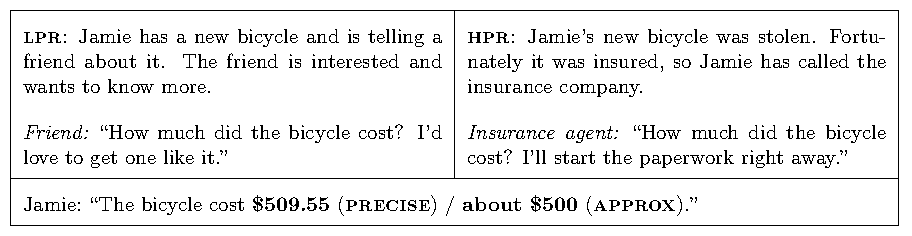
\includegraphics[scale=1.05]{figures/experDesign.pdf}
  \caption{Example scenario (\xvar{lpr}: low precision context; \xvar{hpr}:
           high precision context) with the numerical forms \xvar{precise} and
           \xvar{approx}. This `stolen bike' scenario is one of six pre-tested
           scenarios used in the experiment.}
  \label{fig:bike}
\end{figure}


\subsection{Experimental Results}

All analyses were performed using R \citep{rprogram}, with linear mixed effects
models fitted via \textit{lmerTest} \citep{lmertest}, using form, context, and
their interaction as fixed factors, random intercepts for scenario, and sum
coding for predictors. The results of Task~1 for the attributes \xvar{competent},
\xvar{likeable}, and \xvar{pedantic} are presented in Figure~\ref{figThree}
(mean values and standard deviations).\footnote{The attributes \xvar{knowledgeable},
\xvar{well-prepared}, and \xvar{helpful} showed closely aligned statistics with
\xvar{competent} across all tasks \citep[see][for full results]{soltEtAl2025}.
We therefore exclude them from individual treatment in the SEM evaluation,
treating them as encompassed by \xvar{competent}.}

For \xvar{competent} and \xvar{pedantic}, a significant main effect of form was
found, with \xvar{precise} rated higher ($p < .001$ for both). For
\xvar{competent} and \xvar{likeable}, a significant interaction of context and
form was found: the relative strength of \xvar{precise} versus \xvar{approx} was
greater in \xvar{hpr} than in \xvar{lpr} ($p < .001$ for both). These results
demonstrate that the choice of numerical precision level carries social meaning:
precise speakers score higher on competence-related dimensions compared to
approximate ones, though they are also perceived as more pedantic. These effects
are context-dependent: the positive attributes associated with precise forms are
heightened in high-precision situations, while positive associations with
speaking approximately are more pronounced in low-precision contexts.

\begin{figure}[t!]
  \centering
  \includegraphics[width=\linewidth]{fig4_cs1_empirical_task1}
  \caption{Task~1 rating results (Experiment~1): mean ratings with standard
           deviations for the attributes \xvar{competent}, \xvar{likeable}, and
           \xvar{pedantic}, by numerical form and context. The dashed line marks
           the top of the 7-point rating scale.}
  \label{figThree}
\end{figure}

Figure~\ref{figFreqT2} displays the results of Task~2, showing frequencies of
the 10 most common motivation classes, color-coded by form (blue: approximate,
red: precise). Two coders independently coded the free-text responses; a brief
description of each motivation class is provided in
Figure~\ref{figTask2}(a).

\begin{figure}[t!]
  \centering
  \includegraphics[width=0.75\linewidth]{fig5_cs1_task2_frequencies}
  \caption{Relative frequencies (as a percentage of all participants) of the 10
           most frequently mentioned motivation classes, color-coded by form:
           approximate (blue), precise (red).}
  \label{figFreqT2}
\end{figure}

To explore whether inferred speaker motivations influence social meaning, a
core assumption of SEM, we compared, for each Task~2 motivation class, the
Task~1 ratings of participants who did versus did not mention that class, using
independent-samples $t$-tests (Experiment~1). Figure~\ref{figTask2}(b) displays
the $p$-values for all combinations (3 social attributes $\times$ 10 motivation
classes), with significant effects ($p < .01$) in bold font and direction
indicated by color (green: positive, red: negative). A total of 7 significant
effects were found across 30 combinations, supporting the central SEM assumption
that social meaning is influenced by assumed speaker motivations.

\subsection{Fitting the Model}
To fit SEM to this case study, we construct a scenario model that matches the
experimental design. We define two situational contexts: $c_{LP}$ (low-precision
needs) and $c_{HP}$ (high-precision needs), and two utterance types: $u_{prc}$
(precise) and $u_{apx}$ (explicitly approximate). Figure~\ref{figSketch}
illustrates the model using an analogous scenario in which a speaker reports the
time of an event either precisely (``at 8:32'') or approximately (``around
8:30''), to either a friend at a dinner party or a police officer.

We consider two relevant knowledge states: $k_p$, the speaker has precise
knowledge (e.g., knows the event happened at 8:32), and $k_{\neg p}$, the
speaker has only approximate knowledge (e.g., knows it happened around 8:30
$\pm$ 5 min). The truthfulness function $t$ is defined as $t(k_p) = \{u_{apx},
u_{prc}\}$ and $t(k_{\neg p}) = \{u_{apx}\}$: a speaker with only approximate
knowledge cannot truthfully use a precise utterance. This is shown in
Figure~\ref{figSketch}(a).

We consider three motivation-based strategies, shown in Figure~\ref{figSketch}(b):

\begin{itemize}
  \item $m_{max}$: the speaker is always maximally precise, as long as their
  knowledge state permits it (always precise if $k_p$, approximate if $k_{\neg p}$).
  This captures motivations such as being inherently detail-oriented or wanting
  to convey as much information as possible, regardless of what the situation
  calls for.
  
  \item $m_{sit}$: the speaker matches their precision to the situational demands
  (approximate in $c_{LP}$ and precise in $c_{HP}$, as long as knowledge permits).
  This captures motivations such as judging that a given level of precision is
  appropriate or needed in the situation, or that real-world consequences make
  accuracy important.
  
  \item $m_{min}$: the speaker is always minimally precise regardless of context
  or knowledge. This captures motivations such as habitually preferring
  approximate expressions or finding the approximate form simply easier to
  produce.
  \end{itemize}

%COMMENTS
%GIVE AN INTERPRETATION FOR WHAT THESE STARTEGIES MEAN???


\noindent Figure~\ref{figSketch}(c) illustrates the listener's inferences after
hearing a precise utterance: the listener concludes the speaker has precise
knowledge ($k_p$), and in a high-precision context assigns positive probability
to both $m_{max}$ and $m_{sit}$, while in a low-precision context infers the
speaker follows only $m_{max}$.

\begin{figure}[t!]
  \centering
  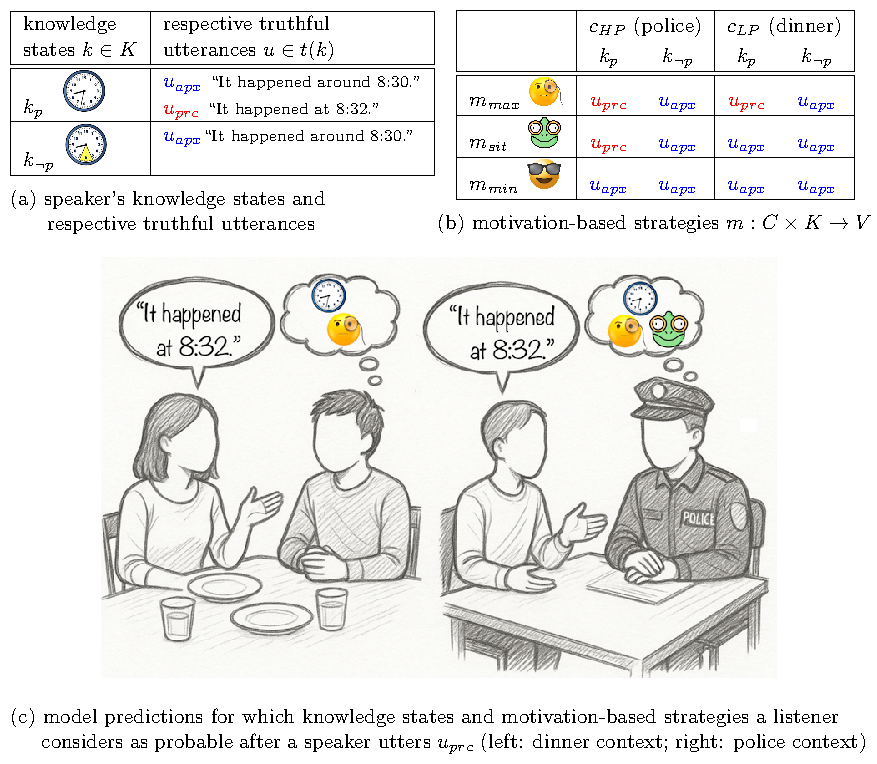
\includegraphics[scale=1.05]{figures/sketchLX.pdf}
  \caption{Exemplary scenario: a speaker reports the time of an event (8:32)
           to a friend at a dinner party (low-precision context) or a police
           officer (high-precision context). (a)~Speaker knowledge states and
           respective truthful utterances. (b)~The three motivation-based
           strategies: $m_{max}$ (always maximally precise), $m_{sit}$
           (situation-adapted), $m_{min}$ (always minimally precise). (c)~Listener
           inferences after hearing a precise utterance, by context.}
  \label{figSketch}
\end{figure}

To fit the impact function $I$, we examine the Task~2 results. The full fitting
procedure is outlined in Figure~\ref{figTask2}. First, we mapped the motivation
classes from Task~2 (Figure~\ref{figTask2}(a)) to model parameters. For
knowledge states: \xvar{knewExact} and \xvar{infoAvail} map to $k_p$;
\xvar{notKnow} and \xvar{infoNotAvail} map to $k_{\neg p}$. For motivation-based
strategies: \xvar{fussyPerson} (inherently precise) maps to $m_{max}$;
\xvar{easySpeaker} and \xvar{usualApx} (consistent approximation for
non-contextual reasons) map to $m_{min}$; \xvar{needed}, \xvar{realWorld}, and
\xvar{purpose} (contextually-sensitive motivations) map to $m_{sit}$. All
mappings are listed in Figure~\ref{figTask2}(c).

The trivalent functions $\phi_K$ and $\phi_M$ are then derived from these
comparisons (Figure~\ref{figTask2}(b)): for each motivation class and attribute
we assign $+1$ for a significant positive difference, $-1$ for a significant
negative difference, and $0$ otherwise (threshold $p < .01$), and replace
motivation class labels with the corresponding model parameters per the mappings
in Figure~\ref{figTask2}(c). Where several motivation classes map to the same
parameter, the cell is set by majority vote. The resulting values are shown in
Figure~\ref{figTask2}(d).\footnote{one cell, $\phi_M(m_{sit})$ on
\xvar{competent}, lies at the significance boundary: the underlying
\xvar{needed}--\xvar{competent} difference is significant under a two-sample
$t$-test ($p = .010$) but falls just short under a mixed-effects model with
random intercepts for scenario ($p = .012$). We retain the $t$-test value; the
model's four qualitative predictions hold under either choice.}

\begin{figure}[t]
  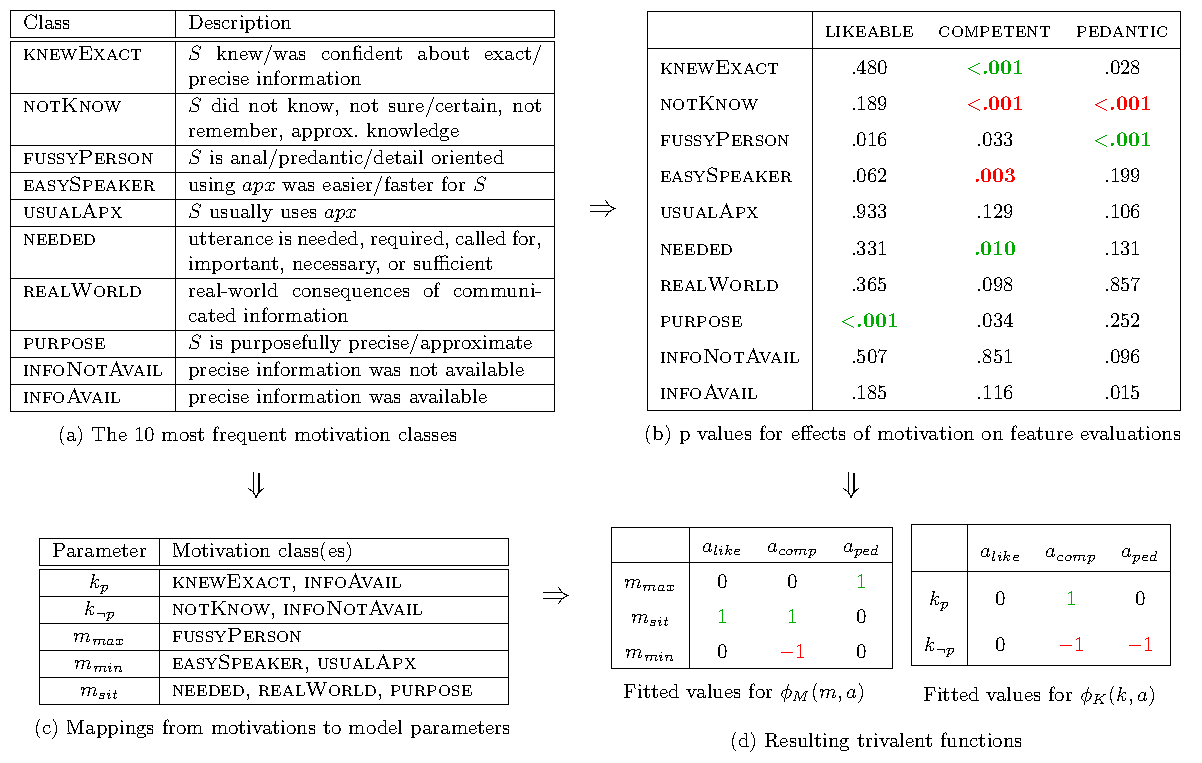
\includegraphics[scale=0.78]{figures/overviewTask2.pdf}
  \caption{(a)~The 10 most frequent motivation classes with descriptions.
           (b)~$p$-values for associations between motivation classes and
           attribute ratings (\xvar{competent}, \xvar{likeable},
           \xvar{pedantic}); significant effects ($p < .01$) in bold,
           green (positive) or red (negative). (c)~Mappings from motivation
           classes to model parameters. (d)~Resulting trivalent functions
           $\phi_K$ and $\phi_M$.}
  \label{figTask2}
\end{figure}


\subsection{Model Predictions}

The fitted SEM has the following free parameters: weight $\omega \in (0,1)$ in
the impact function (Eq.~\ref{eq4}), and the prior probabilities $P(k)$ and
$P(m)$ used to compute the posteriors in Equations~\ref{eq2} and~\ref{eq3}.

For an initial model check, we test a \emph{balanced model}: $\omega = 0.5$
(equal weight to epistemic and motivational inference) and flat prior
probabilities.\footnote{Specifically, $P(m_{max}) = P(m_{sit}) = P(m_{min}) =
\frac{1}{3}$ and $P(k_p) = P(k_{\neg p}) = \frac{1}{2}$.} We then evaluate
the model across a wide range of parameter combinations to assess robustness.

The model check tests whether SEM reproduces the four significant effects from
Experiment~1 (all $p < .001$):

\begin{enumerate}
\item \xvar{precise} is rated higher than \xvar{approx} on \xvar{competent}
across all contexts.

\item \xvar{precise} is rated higher than \xvar{approx} on \xvar{pedantic}
across all contexts.

\item The positive difference between \xvar{precise} and \xvar{approx} on
\xvar{competent} is greater in \xvar{hpr} than in \xvar{lpr}.

\item The relative strength of \xvar{approx} versus \xvar{precise} on
\xvar{likeable} is greater in \xvar{lpr} than in \xvar{hpr}.
\end{enumerate}

SEM is considered qualitatively correct if it reproduces the \emph{direction} of
these effects. To state this precisely, and to introduce two measures we reuse
for the quantitative evaluation in Section~\ref{sec:evaluation}, we summarize
each effect by a signed contrast on the model's evaluation scores. For the two
main effects (1--2) we define, for an attribute $a$, the across-context form
contrast
\[
  \Delta^{\text{main}}_a \;=\; \big[E_L(a|u_{prc}, c_{HP}) + E_L(a|u_{prc}, c_{LP})\big]
  \;-\; \big[E_L(a|u_{apx}, c_{HP}) + E_L(a|u_{apx}, c_{LP})\big],
\]
and for the two interactions (3--4) the context-modulation contrast
\[
  \Delta^{\text{int}}_a \;=\; \big[E_L(a|u_{prc}, c_{HP}) - E_L(a|u_{apx}, c_{HP})\big]
  \;-\; \big[E_L(a|u_{prc}, c_{LP}) - E_L(a|u_{apx}, c_{LP})\big].
\]
Each effect specifies a predicted sign for its contrast: positive for
$\Delta^{\text{main}}_{comp}$ (Effect~1), $\Delta^{\text{main}}_{ped}$
(Effect~2), and $\Delta^{\text{int}}_{comp}$ (Effect~3), and negative for
$\Delta^{\text{int}}_{like}$ (Effect~4).\footnote{Effect~4 is stated as the
\xvar{approx}-over-\xvar{precise} advantage on \xvar{likeable} being greater in
\xvar{lpr} than \xvar{hpr}; written as $\Delta^{\text{int}}_{like}$ above, this
is a negative contrast.} We capture directional agreement with two scores,
following \citet{muehlenbernd2026}:
\[
  \mathrm{DAS} = \frac{\#\{\text{significant main effects with correctly signed } \Delta^{\text{main}}\}}{\#\{\text{significant main effects}\}},
\]
\[
  \mathrm{ISS} = \frac{\#\{\text{significant interactions with correctly signed } \Delta^{\text{int}}\}}{\#\{\text{significant interactions}\}}.
\]
The Directional Agreement Score (DAS) and Interaction Sensitivity Score (ISS)
each range over $[0,1]$, with $1$ indicating that the model reproduces the sign
of every significant effect of the relevant type. SEM is qualitatively correct on
this case study exactly when $\mathrm{DAS} = \mathrm{ISS} = 1$.
\begin{figure}[t!]
  \centering
  \includegraphics[width=\linewidth]{fig8_cs1_model_vs_empirical}
  \caption{Predictions of the balanced model for the attributes \xvar{competent},
           \xvar{likeable}, and \xvar{pedantic} (top row, evaluation scores
           $E_L \in [-1, 1]$), shown alongside the empirical results of
           Experiment~1 (bottom row, mean ratings linearly rescaled to $[-1, 1]$
           via $(x-4)/3$). Bars rise from the scale floor ($-1$, the lowest
           evaluation); $0$ denotes a median, not neutral, evaluation.}
  \label{ficPred}
\end{figure}
Figure~\ref{ficPred} presents the balanced model's predictions for $a_{comp}$,
$a_{like}$, and $a_{ped}$ across utterances and contexts, alongside the empirical
results. The balanced model achieves $\mathrm{DAS} = \mathrm{ISS} = 1$,
reproducing the sign of all four significant effects, and the attribute-internal
patterns are visibly aligned with the empirical data.

To assess robustness, we tested the balanced model against an exhaustive grid of
free parameter combinations: every combination of $\omega$ (from 0.05 to 0.95)
and the prior probabilities $P(k_p)$, $P(k_{\neg p})$, $P(m_{max})$,
$P(m_{sit})$, and $P(m_{min})$ (from 0 to 1), each in increments of 0.02,
yielding 2,593,080 valid combinations. 
SEM achieves $\mathrm{DAS} = \mathrm{ISS} = 1$ for $99.87\%$ of combinations; for
the remaining $0.13\%$ one of the four effects flips sign (always within the main
effects, so $\mathrm{ISS} = 1$ throughout).\footnote{In particular, the model struggled to predict
Effect~1 correctly when $\omega$ was very low, $P(k_p)$ was very low, and
$P(m_{sit})$ was high, a combination of parameters that is difficult to
motivate on independent grounds.} This demonstrates the robustness of the
qualitative predictions across the free parameter space.

Section~\ref{sec:evaluation} presents a quantitative evaluation of these
predictions, comparing the full model against simplified variants (referred to
as \emph{ablations}), in which individual inferential components are removed
one at a time, to assess which components are necessary to reproduce the
empirical patterns.




% -----------------------------------------------------------------------------
\section{Quantitative Evaluation and Model Comparison}
\label{sec:evaluation}
% -----------------------------------------------------------------------------

The preceding sections established that SEM qualitatively reproduces the four
significant empirical effects from Experiment~1 across almost all free parameter
settings (99.87\% of 2,593,080 combinations). This section asks a deeper
question: \emph{how well} does the model reproduce those effects, and does its
formal inference machinery add explanatory value over simpler alternatives?

We address this with two analyses. First, we evaluate the balanced model's
quantitative fit against the empirical means using an established metric suite.
Second, we compare the full model against three nested ablations, each of which
removes one inferential component, evaluated across a sample of parameter
combinations rather than a single setting, so that differences reflect structural
properties of the model variants rather than parameter choices.


\subsection{Metric Framework}
\label{sec:metrics}

Quantitative model evaluation follows the framework proposed by
\citet{muehlenbernd2026} for assessing probabilistic pragmatic models against
human data. We compare model scores $E_L(a|u,c) \in [-1,1]$ against empirical
human means, which are linearly rescaled from the 7-point Likert scale to
$[-1,1]$ via $(x-4)/3$, making model and human values directly comparable.

For an attribute $a$, let $\Delta_{H,a}$ and $\Delta_{M,a}$ denote the human
and model contrast values (the $\Delta^{\text{main}}_a$ or $\Delta^{\text{int}}_a$
of Section~\ref{sec:imprecision}, as appropriate). We report three metrics:

\begin{itemize}
\item \textbf{DAS} (Directional Agreement Score) and \textbf{ISS} (Interaction
Sensitivity Score): as defined in Section~\ref{sec:imprecision}: the proportion
of significant main effects, respectively significant form $\times$ context
interactions, on which model and human agree in sign. Range $[0,1]$.

\item \textbf{CDS} (Calibration Deviation Score): mean $|\text{ESR} - 1|$ across
significant effects, where ESR (Effect Size Ratio) $= |\Delta_{M,a}| /
|\Delta_{H,a}|$ for each significant effect.\footnote{ESR $= 1$ indicates
perfect magnitude calibration; ESR $> 1$ means the model overshoots the human
contrast; ESR $< 1$ means it undershoots. CDS aggregates these per-effect
deviations: lower is better, with $0$ indicating perfect magnitude calibration.
ESR is computed only for significant effects to avoid division by near-zero
human contrasts.} Lower is better; $0$ = perfect magnitude calibration.
\end{itemize}

DAS, ISS, and CDS are computed over the four effects that are statistically
significant in the human data: the main effects of form on $a_{comp}$ and
$a_{ped}$, and the form $\times$ context interactions on $a_{comp}$ and
$a_{like}$. The remaining two of the six possible effects, the main effect on
$a_{like}$ and the interaction on $a_{ped}$, are non-significant and are not
assessed, since testing directional agreement or magnitude calibration on a
near-zero human contrast would treat noise as signal. For the model variant
comparison in Section~\ref{sec:variants}, we additionally report \textbf{RMSE}
(root mean squared error), computed cell-by-cell over all 12 condition means
(3 attributes $\times$ 2 forms $\times$ 2 contexts) after rescaling human means
to $[-1,1]$. RMSE gives a global picture of fit across the full data surface
and is particularly informative when comparing variants that differ in their
overall prediction patterns.


\subsection{Balanced Model Fit}
\label{sec:balancedfit}

Table~\ref{tab:balanced_fit} reports the metric set for the balanced model
($\omega = 0.5$, flat priors). DAS and ISS are included for completeness but,
as both equal $1.00$, were already discussed in Section~\ref{sec:imprecision};
the focus here is on the calibration metrics.

\begin{table}[t!]
\centering
\caption{Quantitative fit of the balanced model ($\omega=0.5$, flat priors)
         against empirical means from Experiment~1 ($N=362$). DAS, ISS, and
         CDS are computed over the four statistically significant effects only.}
\label{tab:balanced_fit}
\begin{tabular}{lc}
\toprule
Metric & Value \\
\midrule
DAS              & 1.00 \\
ISS              & 1.00 \\
CDS (main)        & 1.19 \\
CDS (interaction) & 0.31 \\
CDS (overall)     & 0.75 \\
\bottomrule
\end{tabular}
\end{table}

The calibration metrics reveal a systematic pattern the directional check cannot
see. The balanced model overshoots effect magnitudes on the main effects: CDS
(main) $= 1.19$ indicates that on average the model predicts roughly twice the
human contrast for $a_{comp}$ and $a_{ped}$. Calibration on the interactions is
markedly better (CDS (interaction) $= 0.31$); that is, the model is best
calibrated precisely where its context-sensitive reasoning does the most work,
and overshoots on the simpler main effects.

The magnitude overshoot on main effects is a property of the balanced parameter
setting rather than a structural limitation of the model. A grid search over the
free parameter space identifies a setting ($\omega = 0.7$, $P(k_p) = 0.9$,
$P(m_{max}) = 0.5$, $P(m_{sit}) = 0.3$, $P(m_{min}) = 0.2$) that achieves
near-perfect calibration (CDS $= 0.056$; RMSE $= 0.165$), while preserving
$\mathrm{DAS} = \mathrm{ISS} = 1.00$. This confirms that the overshoot under
balanced parameters reflects the uninformative prior choice, not an architectural
flaw.\footnote{This is an in-sample, post-hoc result: the optimized parameters
are tuned to the same 12 data cells from which the impact functions were derived,
so it represents an upper bound on fit rather than a validated generalization.
The balanced model is the primary evaluation throughout; the grid search result
is reported as a calibration bound.}


\subsection{Model Variant Comparison}
\label{sec:variants}

A central question for any model of this kind is whether its inference machinery
adds explanatory value beyond simpler alternatives. We address this by asking
which of SEM's inferential components are necessary to reproduce the empirical
pattern, comparing the full model against three nested ablations, each of which
removes one inferential component while holding everything else equal:

\begin{itemize}
\item \textbf{SEM-full}: the complete model, all parameters free.
\item \textbf{SEM-context-blind}: $P(m_{sit}) = 0$, removing the
context-sensitive motivation strategy. This operationalizes a
``violation-of-expectation'' account in which the model can infer knowledge
states and non-contextual motivations, but has no mechanism for context to
modulate evaluations positively.
\item \textbf{SEM-knowledge-only}: $\omega = 1$, so only epistemic inference
contributes to evaluation. Motivation inference is disabled entirely.
\item \textbf{SEM-motivation-only}: $\omega = 0$, so only motivational inference
contributes. Knowledge-state inference is disabled entirely.
\end{itemize}

To make the comparison robust to parameter choice, each variant is evaluated
across 100 sampled parameter combinations rather than a single setting. Free
parameters are drawn from uninformative distributions ($\omega \sim
\text{Beta}(2,2)$ clipped to $(0.05, 0.95)$; $P(k) \sim \text{Dirichlet}(1,1)$;
$P(m) \sim \text{Dirichlet}(1,1,1)$; seed fixed for reproducibility), and
metrics are computed for each draw. We report mean $\pm$ standard deviation
across draws. A difference that is consistent across the full sample reflects
a structural property of the model variant, not a parameter artifact.

Table~\ref{tab:variant_comparison} reports the results.

\begin{table}[ht]
\centering
\caption{Quantitative comparison of four SEM variants across 100 sampled
         parameter combinations (mean $\pm$ SD). DAS, ISS, and CDS are
         computed over the four significant effects only; RMSE over all 12
         conditions. Lower CDS and RMSE are better; higher ISS and DAS are
         better.}
\label{tab:variant_comparison}
\renewcommand{\arraystretch}{1.15}
\begin{tabular}{lcccc}
\toprule
Metric & SEM-full & Context-blind & Know-only & Motiv-only \\
\midrule
DAS            & $1.00 \pm 0.00$ & $1.00 \pm 0.00$ & $1.00 \pm 0.00$ & $0.96 \pm 0.13$ \\
ISS            & $\mathbf{1.00 \pm 0.00}$ & $0.00 \pm 0.00$ & $0.04 \pm 0.14$ & $1.00 \pm 0.00$ \\
RMSE           & $\mathbf{0.30 \pm 0.10}$ & $0.42 \pm 0.12$ & $0.39 \pm 0.14$ & $0.51 \pm 0.09$ \\
CDS (main)     & $\mathbf{1.06 \pm 0.71}$ & $1.46 \pm 0.72$ & $1.65 \pm 1.25$ & $1.07 \pm 0.56$ \\
CDS (inter)    & $\mathbf{0.82 \pm 0.62}$ & $1.00 \pm 0.00$ & $1.00 \pm 0.00$ & $1.79 \pm 1.44$ \\
CDS (overall)  & $\mathbf{0.94 \pm 0.43}$ & $1.23 \pm 0.36$ & $1.32 \pm 0.62$ & $1.43 \pm 0.67$ \\
\bottomrule
\end{tabular}
\end{table}

The key finding is ISS: it collapses to $\approx 0$ for the two variants that
remove $m_{sit}$ (context-blind: $0.00$; knowledge-only: $0.04$) and stays at
$1.00$ for the two that retain it (full and motivation-only). Since the two
significant interaction effects are precisely the form $\times$ context effects
captured by $m_{sit}$, this means context-blind and knowledge-only cannot
reproduce two of the four significant empirical effects at all, regardless of
parameter setting. The context-sensitive motivation mechanism is structurally
necessary, not a decorative feature of the model.

Each ablation fails on a distinct dimension, and none matches the full model on
both structure and calibration. The context-blind variant loses the interactions
entirely (ISS $= 0$) and also degrades on RMSE ($0.30 \to 0.42$) and overall
CDS ($0.94 \to 1.23$). The motivation-only variant keeps the interaction
directions (ISS $= 1.00$) but is otherwise the weakest: it massively overshoots
interaction magnitudes (CDS interaction $= 1.79$) and has the highest RMSE
($0.51$), because without knowledge inference the competence ordering breaks
down. The knowledge-only variant achieves the second-lowest RMSE ($0.39$),
reflecting that the study's overall ordering is largely epistemic: precise
speakers are inferred to have precise knowledge, which is the dominant signal in
the data. But its ISS of $0.04$ means it fails entirely on the interactions.
Without motivational inference, the model cannot represent context as modulating
the epistemic ordering, and so it misses two of the four significant empirical
effects regardless of parameter setting. A model that reproduces the main trend
while missing the context-sensitivity has not captured the phenomenon.

Taken together, the full SEM is the only variant that reproduces the interaction
structure (ISS $= 1.00$) while remaining competitive on global fit (lowest RMSE,
lowest overall CDS). Every simpler alternative either matches or exceeds it on
one metric while failing conspicuously on another. This pattern provides
direct evidence that the model's staged inference, from epistemic state through
contextual motivation, to social attribute, is necessary rather than redundant.

The CDS results also bear on the question of magnitude calibration raised
above. The interaction CDS difference between the full model ($0.82$) and the
ablations that lose $m_{sit}$ (both pinned at $1.00$, since their predicted
interaction contrasts are zero) quantifies the specific contribution of
contextual motivation inference to calibration. The full model's main-effect CDS
($1.06$) is essentially tied with the motivation-only variant ($1.07$),
confirming that main-effect overshoot is a shared property of the trivalent
impact scale and not specific to any particular model configuration.

\paragraph{The symmetry of the two inferential dimensions.}
It would be a misreading of these results to conclude that one inferential
component is more fundamental than the other. The ablations show that for
\emph{this} phenomenon both the epistemic and the motivational dimension are
required, but they do not rank the two: knowledge-only fails on the interactions
(ISS) and motivation-only fails on calibration, because numerical (im)precision
happens to load on both dimensions at once, the epistemic dimension securing the
competence ordering and the motivational dimension securing its context-sensitivity.

Other phenomena need not be balanced in this way. SEM can represent a phenomenon
in which either dimension is inert, and it can do so in two ways that require no
change to the model definition. One is through the weight: setting $\omega = 1$
or $\omega = 0$ removes the motivational or the epistemic contribution to the
impact function, respectively, which is exactly what the knowledge-only and
motivation-only ablations do. The other, and more natural where a distinction is
simply irrelevant, is through the inference domains themselves: a phenomenon in
which the speaker's knowledge is not at issue is modeled with a single knowledge
state ($|K| = 1$), and one in which no motivational distinction is relevant with a
single strategy ($|M| = 1$). In either case the corresponding inference becomes
vacuous and the social evaluation is driven entirely by the other dimension. A
purely epistemic phenomenon, such as the social uptake of a scalar implicature,
where what matters is whether the speaker is taken to know the stronger
alternative, would be a natural $|M| = 1$ case; a phenomenon in which the
speaker's knowledge is not in question but their communicative motivation is, as
in some politeness and register choices (Section~\ref{sem-extension}), would be a
natural $|K| = 1$ case. The full SEM is required for (im)precision not because the
architecture privileges any one route, but because this particular phenomenon
exercises both.


\paragraph{Threshold robustness.}
The $\phi$ functions are derived at $p < .01$. Re-running the full comparison
with $\phi$ derived at $p < .05$ (which adds three non-zero cells) worsens the
full model on every calibration metric (CDS $0.94 \to 1.45$, RMSE $0.30 \to
0.51$) while leaving ISS unchanged. Tightening to $p < .001$ slightly improves
CDS ($0.94 \to 0.89$) but degrades interaction coverage (ISS $1.00 \to 0.57$)
because the borderline $m_{sit}$--$a_{comp}$ cell is dropped. The $p < .01$
threshold is the only one that maintains full interaction coverage while
achieving competitive calibration.\footnote{These threshold comparisons were
conducted by re-deriving $\phi_K$ and $\phi_M$ at each threshold from the same
Experiment~1 data and re-running the variant comparison. Scripts are available
in the repository.}


% -----------------------------------------------------------------------------
\section{Discussion and Conclusion}
\label{sec:conclusion}
% -----------------------------------------------------------------------------

\subsection{Summary of Contributions}

The Social Evaluation Model (SEM) is a probabilistic framework that explains
how listeners form social impressions of speakers based on their pragmatic
behavior, integrating cognitive, epistemic, and social reasoning within a
unified formal architecture. By extending the inferential chain of probabilistic
pragmatics, SEM shows how linguistic choices, such as the level of numerical
precision, give rise to evaluations of traits like competence, warmth, and
pedantry through staged Bayesian inference. The model accurately reproduces the
key empirical patterns from a matched-guise study on numerical (im)precision: it
predicts how varying levels of precision affect competence, likeability, and
pedantry ratings as a function of contextual demands, and the quantitative
evaluation demonstrates that its staged inference architecture, from epistemic
state through contextual motivation, to social attribute, is necessary to
reproduce the observed pattern. The simplified variants show that no single component of the model can carry
the full explanatory load: each variant reproduces some of the empirical
pattern but fails on a distinct aspect of it. Most tellingly, removing the
context-sensitive motivation strategy makes the model blind to how context
shapes social evaluations, collapsing its ability to capture the interaction
effects entirely. Together, these comparisons provide direct evidence that the
model's staged inference architecture, proceeding from epistemic state through
contextual motivation to social attribute, reflects genuine structure in the
data rather than an arbitrary modeling choice.

\subsection{Extending SEM to Other Social-Meaning Phenomena}
\label{sem-extension}

Although we have developed and tested SEM on a single phenomenon, numerical
(im)precision, its architecture is not specific to that domain. SEM has the 
potential to serve as a modeling framework wherever three
conditions hold: a speaker chooses among non-equivalent alternatives, that
choice supports inferences about the speaker's knowledge state and communicative
motivation, and those inferences in turn bear on the listener's social
evaluation of the speaker. A number of well-studied
phenomena meet these conditions, and we sketch several here as candidates for
future modeling.

The most direct extension is to the pragmatic violations studied by
\citet{beltramapapafragou2023}, who show that a speaker's adherence to or
violation of the Gricean maxims of Relevance and Informativeness shifts listeners'
evaluations of the speaker's warmth and competence, and, crucially, that the
\emph{reason} attributed to a violation modulates this effect: an uninformative
answer attributed to inability is evaluated differently from one attributed to
unwillingness. This is precisely the structure SEM formalizes. The alternatives
are the relevant versus irrelevant, informative versus uninformative responses;
the knowledge states distinguish a speaker who cannot be informative from one who
can; and the motivation strategies capture why a speaker would withhold relevant
information. A SEM treatment would capture this distinction naturally: inability maps onto
a knowledge state in which the speaker lacks the relevant information, while
unwillingness maps onto a motivation-based strategy of withholding it, each
with different impact-function signatures on warmth and competence, yielding
the asymmetry Beltrama and Papafragou observe.
Because their study elicits social-attribute ratings on the same warmth and
competence dimensions used here, it is well suited to the quantitative evaluation
of Section~\ref{sec:evaluation}.

Politeness and indirect speech offer a second candidate. A speaker who chooses an
indirect or mitigated form over a direct one invites inferences about their
motives, deference, face-management, or self-presentation, that feed social
evaluation \citep{brownlevinson1987,LeePinker2010}. Probabilistic models of
polite language already treat such choices as arising from competing
informational and social goals: in \citeauthor{yoontessleretal2020}'s
(\citeyear{yoontessleretal2020}) model, a speaker selects utterances partly to
manage how they will be perceived, treating \emph{self-presentation} as an
explicit production goal. This is revealing for SEM, because a speaker's
self-presentation goal just is an anticipation of the social evaluation a
listener will form: the speaker reasons about the very inference that SEM models
on the listener's side. The two models thus describe complementary halves of a
single social-pragmatic loop, the speaker choosing a form in anticipation of
being evaluated, the listener evaluating on the basis of that choice, and SEM
supplies the listener-side component that a self-presenting speaker must
implicitly represent. We return to this speaker--listener integration in
Section~\ref{sec:rsa-int}.

A third candidate is the use of \emph{hedging} and uncertainty expressions (e.g.,
\emph{I think}, \emph{probably}, \emph{might}). The choice between a hedged and an
unhedged assertion is a choice among non-equivalent alternatives that supports
inferences about the speaker's epistemic state and their motivation for marking
it, and these inferences carry social weight. \citet{mccready2015} analyzes
hedging precisely as a reputation-management device: speakers hedge to protect
their standing for cooperativity against the cost of an assertion that may turn
out to be unwarranted. Cast in SEM's terms, this is a motivation strategy whose
impact-function signature trades perceived competence (a confident, unhedged
assertion projects knowledge) against the social protection a hedge affords if
the speaker is wrong, with the social outcome depending on which motivation the
listener infers. Listeners are demonstrably sensitive to such variation and adapt
to speaker-specific patterns of uncertainty marking \citep{schusterdegen2020},
which also makes hedging a natural site for studying the listener variation that
SEM's free parameters are designed to represent.

A fourth candidate, drawn from a different grammatical domain, is honorification
and register. \citet{mccready2019} analyzes honorifics as encoding the formality
a speaker takes to be appropriate to the speech situation; the choice among
register levels is thus a context-sensitive selection among alternatives that
conveys social meaning. Where an honorific form is over- or under-used relative to
situational expectations, listeners draw inferences about the speaker's stance,
deference, or social competence, an inferential step of exactly the kind SEM
models, though here the relevant attributes (e.g., respectfulness, social
fluency) and the role of situational context differ from the precision case.

What unites these phenomena is the structure SEM is built to capture: a choice
among meaningful alternatives, interpreted through inferences about what the
speaker knows and why they chose as they did, issuing in a social evaluation.
Establishing SEM's generality across them, ideally with the same quantitative
methodology applied here, is a central goal for future work.

\subsection{Relation to the RSA Framework}

Section~\ref{sec:sem} introduced SEM as an extension of the RSA inferential
chain rather than a competitor to it. We now develop that relationship in more
detail, since it bears on a recurring question about the model: is a new model
needed at all, or could the existing RSA architecture simply be extended to
cover social evaluation? Our answer is that the extension is real but
substantive, it requires machinery that standard RSA does not contain, and that
SEM and RSA are naturally compatible rather than opposed. The remainder of this
subsection makes the points of contact and departure explicit.

RSA is a framework for modeling how communicative meaning is derived through
recursive reasoning about speaker and listener mental states. In standard RSA,
the speaker selects utterances to maximize a utility function, typically a
function of informational value and cost; the listener uses Bayes' rule to invert
this speaker model and recover the intended meaning. Social goals can be
incorporated into the utility function, as in \citeauthor{yoontessleretal2020}'s
(\citeyear{yoontessleretal2020}) model of polite speech, which treats politeness
as a competing goal alongside informativeness. This shows that RSA can be
extended to encompass some aspects of social reasoning, and we take this as an
important point of contact.

SEM differs, however, in its architecture and target of inference. First, SEM
models social evaluation from the \emph{listener's} perspective, whereas RSA
typically models the speaker's production choices. In SEM, the listener's
inferential process yields a social evaluation as its output; the model does not
make claims about how speakers optimize their utterances (though see below for
how SEM and RSA can be integrated). Second, SEM replaces the continuous utility
function of RSA with a discrete set of behavioral strategies, each representing a
recognizable communicative motivation. This design choice makes the strategies
directly groundable in empirical data, specifically in the motivation classes
that participants attribute to speakers in free-text tasks, and makes the model's
parameters interpretable and testable. A utility-based extension of RSA could
also include social attributes as latent variables, but the mapping from
utilities to the behavioral diversity captured by SEM's motivation strategies
would need to be explicitly specified. Third, the impact function $I$ and the
fitted trivalent functions $\phi_K$ and $\phi_M$ have no counterpart in standard
RSA. They constitute the formal machinery for linking pragmatic inference to
social evaluation, and their empirical grounding is a methodological contribution
distinct from RSA extensions.

Taken together, SEM is best understood not as an alternative to RSA but as a
complementary module that extends the inferential chain one step further: from
what the speaker meant, to what kind of communicator they are.


\subsection{Relation to the Social Meaning Games framework}

SEM also relates to the Social Meaning Games framework (SMG)
\citep{burnett2017,burnett2019,burnett2023}. SMG models strategic reasoning
over an indexical field that is taken as given: speakers choose among variants
to construct a persona that maximizes their expected utility given their
beliefs about how listeners will interpret each variant, and listeners use
Bayesian updating over the same field to infer the speaker's persona from
their choice of variant. This reasoning step is genuine and, like SEM's,
listener-oriented: the same variant can receive different social
interpretations depending on a listener's prior beliefs about the particular
speaker, a pattern \citet{burnett2019} models directly for sociophonetic
variables such as (ING) and released~/t/. What SMG does not derive is the
indexical field itself: the mapping between a variant and the properties it
can signal is stipulated as part of the model's input, and how such mappings
are acquired or change over time is explicitly left as a direction for future
work \citep{burnett2019}.

SEM and SMG are complementary in the kind of reasoning they formalize 
and the types of social meaning they are designed to capture. SMG is
designed for semantically equivalent variants whose indexical field is
established by convention (e.g., sociophonetic variation such as ING); given
that field, it models how a listener infers a speaker's persona via Bayesian
reasoning over a fixed, stipulated mapping between linguistic forms and social
properties. SEM is designed for semantically non-equivalent alternatives,
where the listener's reasoning is not anchored to a conventionalized field but
derived from the truthfulness constraint and the structure of the alternatives
themselves: it models how differences in semantic content or pragmatic choice
lead listeners to infer a speaker's knowledge state and motivation, and from
these, specific social attributes. Put differently, SMG explains how speakers
and listeners coordinate on an already-established system of social meaning;
SEM explains how social meaning can be derived from pragmatic reasoning even
where no such system is presupposed.


\subsection{Limitations}
Several limitations of the current formulation are worth noting. The trivalent
functions $\phi_K$ and $\phi_M$ make a simplifying assumption: that a given
knowledge state or motivation-based strategy has a fixed, consistent impact on a
social attribute regardless of context. In reality, the underlying motivations
corresponding to a single behavioral strategy may differ in their social
implications. A more refined model would include an additional inference step
recovering the probability of each specific motivation given a strategy; we leave
this generalization to future work. The current model has been evaluated on a
single empirical case study (numerical imprecision); the framework's
applicability to other pragmatic domains, for example politeness phenomena or
relevance violations, is a natural direction for future empirical work.

A further simplification concerns the set of social attributes $A$ itself. SEM
takes $A$ to be a finite set supplied by the modeler, here the attributes
elicited in the experiment, but in principle the attributes a listener might
ascribe to a speaker are open-ended. The model is agnostic about which attributes
populate $A$: any attribute for which the impact functions $\phi_K$ and $\phi_M$
can be specified (whether fitted from data or stipulated) can be added without
change to the architecture. What SEM does not currently model is how listeners
select or generate the relevant attributes in the first place; we take the
attribute set as given and model the inference from utterance to evaluation along
it.

A limitation of the current formulation concerns the structure of listener
variation. As noted in Section~\ref{sec:sem}, the priors and weight $\omega$
already encode listener-level variation, and the parameter sampling in
Section~\ref{sec:variants} treats a spread of settings as a population of
listeners. What this does not capture is \emph{systematic} variation: for
instance, speaker-specific priors arising from the sensitivity of comprehension
to speaker identity, or differences in $\omega$ tied to listener traits or social
relationships. Such structure could be incorporated by conditioning the priors
or the weight on listener- and speaker-level covariates, and modeling how these
are themselves inferred; we leave this to future work.

\subsection{Integration with RSA and Future Directions}
\label{sec:rsa-int}

Looking forward, SEM can be naturally integrated into higher-order models of
pragmatic reasoning such as RSA. In such an integrated model, the outcomes of
SEM, listeners' judgments of competence, warmth, or sincerity, become part of
the speaker's production process: speakers could anticipate the evaluative
inferences their utterances are likely to elicit, and strategically choose
expressions that present them favorably. This connects pragmatic reasoning to
social signaling and impression management, framing communication as recursive
social cognition in which agents reason continuously about both the informational
and social consequences of their linguistic choices. Developing this integration
formally, and testing its predictions empirically, is a central direction for
future research.

\bigskip

\noindent\textbf{Data and code availability.}
The experimental data and R analysis scripts are available on the Open Science
Framework at \url{[ANONYMIZED OSF PROJECT LINK]}; the preregistration for
Experiment~1 is at \url{[ANONYMIZED OSF PREREG LINK]}. A Python implementation of
SEM, including a Jupyter notebook that reproduces all analyses and figures
reported here, is available at \url{[ANONYMIZED GITHUB REPO LINK]}.


% -----------------------------------------------------------------------------
\printbibliography
% -----------------------------------------------------------------------------

\end{document}
